\documentclass{article}%
\usepackage[T1]{fontenc}%
\usepackage[utf8]{inputenc}%
\usepackage{lmodern}%
\usepackage{textcomp}%
\usepackage{lastpage}%
\usepackage{geometry}%
\geometry{left=2.5cm,top=1.5cm}%
\usepackage[dvipsnames]{xcolor}%
\usepackage{array}%
\usepackage{colortbl}%
\usepackage{graphicx}%
\usepackage{caption}%
\usepackage{slashbox}%
\usepackage{ragged2e}%
\usepackage{tcolorbox}%
\usepackage{booktabs}%
%
%
%
\begin{document}%
\normalsize%
\section{Análsis Sísmico}%
\label{sec:AnlsisSsmico}%
Esto mostrará una lista de los commits en el repositorio, comenzando con el commit más reciente. Cada commit estará identificado por una cadena de caracteres larga y hexadecimal que aparece en la línea que comienz%
\subsection{Parámetros de Sitio}%
\label{subsec:ParmetrosdeSitio}%
\subsubsection{Factor de Zona}%
\label{ssubsec:FactordeZona}%
Esto mostrará una lista de los commits en el repositorio, comenzando con el commit más reciente.\newline%
Cada commit estará identificado por una cadena de caracteres larga y hexadecimal que aparece en la\newline%
línea que comien\newline%
%


\begin{table}[ht!]%
\begin{minipage}{0.55\textwidth}%
\caption{Factor de zona}%
\begin{tabular}{|>{\centering\arraybackslash}m{3.75cm}|>{\centering\arraybackslash}m{3.75cm}|}%
\hline%
\multicolumn{2}{|c|}{\textbf{FACTOR DE ZONA SEGÚN E{-}030}}\\%
\hline%
\textbf{ZONA}&\textbf{Z}\\%
\hline%
4&0.45\\%
\hline%
3\cellcolor[rgb]{ .949,  .949,  .949} &\textcolor[rgb]{ 1,  0,  0}{\textbf{0.35}}\cellcolor[rgb]{ .949,  .949,  .949} \\%
\hline%
2&0.25\\%
\hline%
1&0.10\\%
\hline%
\end{tabular}%
\end{minipage}%
\begin{minipage}{0.35\textwidth}%
\begin{center}%
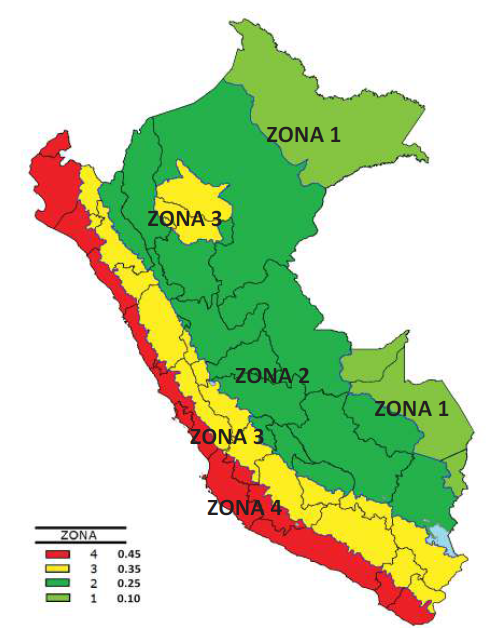
\includegraphics[width=4cm]{mapa_zona}%
\end{center}%
\end{minipage}%
\caption*{Fuente: E-30 (2018)}%
\end{table}

%
\subsubsection{Factor de suelo}%
\label{ssubsec:Factordesuelo}%
%


\begin{table}[ht!]%
\centering%
\caption{Factor de zona}%
\begin{tabular}{|>{\centering\arraybackslash}m{3.75cm}|>{\centering\arraybackslash}m{2cm}|>{\centering\arraybackslash}m{2cm}|>{\centering\arraybackslash}m{2cm}|>{\centering\arraybackslash}m{2cm}|}%
\hline%
\multicolumn{5}{|c|}{\textbf{FACTOR DE SUELO SEGÚN E{-}030}}\\%
\hline%
\backslashbox{\textit{\textbf{ZONA}}}{\textit{\textbf{SUELO}}}&\textbf{S0}&\textbf{S1}&\textbf{S2}&\textbf{S3}\\%
\hline%
4&0.80\cellcolor[rgb]{ .949,  .949,  .949} &1.00&1.05&1.10\\%
\hline%
3\cellcolor[rgb]{ .949,  .949,  .949} &\textcolor[rgb]{ 1,  0,  0}{\textbf{0.80}}\cellcolor[rgb]{ .949,  .949,  .949} \cellcolor[rgb]{ .949,  .949,  .949} &1.00\cellcolor[rgb]{ .949,  .949,  .949} &1.15\cellcolor[rgb]{ .949,  .949,  .949} &1.20\cellcolor[rgb]{ .949,  .949,  .949} \\%
\hline%
2&0.80\cellcolor[rgb]{ .949,  .949,  .949} &1.00&1.20&1.40\\%
\hline%
1&0.80\cellcolor[rgb]{ .949,  .949,  .949} &1.00&1.60&2.00\\%
\hline%
\end{tabular}%
\caption*{Fuente: E-30 (2018)}%
\end{table}

%
\section{Irregularidades}%
\label{sec:Irregularidades}%
\subsubsection{Irregularidad Torsional}%
\label{ssubsec:IrregularidadTorsional}%
\begin{tcolorbox}[colback=gray!5!white,colframe=cyan!75!black,fonttitle=\bfseries,title=Tabla N°9 E-030]%
Existe irregularidad torsional cuando, en cualquiera de las direcciones de análisis el desplazamiento relativo de entrepiso en un edificion ($\Delta_{max}$) en esa dirección, calculado incluyendo excentricidad accidental, es mayor que 1,3 veces el desplazamineto relativo promedio de los extremos del mismo entrepiso para la condicion de carga ($\Delta_{prom}$). 
 Este crriterio sólo se aplica en edificios con diafragmas rígidos y sólo si el máximo desplazamiento relativo de entrepiso es mayor que 50\% del desplazamiento permisible indicado en la Tabla N° 11%
\end{tcolorbox}%
\begin{tcolorbox}[colback=gray!5!white,colframe=cyan!75!black,fonttitle=\bfseries,title=Tabla N°9 E-030]%
Existe irregularidad torsional cuando, en cualquiera de las direcciones de análisis el desplazamiento relativo de entrepiso en un edificion ($\Delta_{max}$) en esa dirección, calculado incluyendo excentricidad accidental, es mayor que 1,3 veces el desplazamineto relativo promedio de los extremos del mismo entrepiso para la condicion de carga ($\Delta_{prom}$). 
 Este crriterio sólo se aplica en edificios con diafragmas rígidos y sólo si el máximo desplazamiento relativo de entrepiso es mayor que 50\% del desplazamiento permisible indicado en la Tabla N° 11%
\end{tcolorbox}%
%


\begin{table}[ht!]%
\centering%
\caption{Irregularidad Torsional}%
\resizebox{\textwidth}{!}{%
\begin{tabular}{cccccccccc}
\toprule
Story & OutputCase & Direction & Max Drift & Avg Drift & Ratio & Height & Drifts & < Driftmax/2 & Es Regular \\
\midrule
Story8 & SDx Max & X & 0.003021 & 0.002475 & 1.221 & 2.5 & 0.006344 & False & Regular \\
Story7 & SDx Max & X & 0.003476 & 0.002869 & 1.211 & 2.5 & 0.007300 & False & Regular \\
Story6 & SDx Max & X & 0.004116 & 0.003335 & 1.234 & 2.5 & 0.008644 & False & Regular \\
Story5 & SDx Max & X & 0.00454 & 0.003673 & 1.236 & 2.5 & 0.009534 & False & Regular \\
Story4 & SDx Max & X & 0.004657 & 0.003773 & 1.234 & 2.5 & 0.009780 & False & Regular \\
Story3 & SDx Max & X & 0.004479 & 0.003582 & 1.25 & 2.5 & 0.009406 & False & Regular \\
Story2 & SDx Max & X & 0.003811 & 0.002958 & 1.288 & 2.5 & 0.008003 & False & Regular \\
Story1 & SDx Max & X & 0.001124 & 0.000904 & 1.244 & 1.5 & 0.003934 & False & Regular \\
NT & SDx Max & X & 0.00024 & 0.00012 & 2 & 1.75 & 0.000720 & True & Regular \\
NT & SDx Max & Y & 2.8E-05 & 1.4E-05 & 2 & 1.75 & 0.000084 & True & Regular \\
\bottomrule
\end{tabular}
}%
\end{table}

%


\begin{table}[ht!]%
\centering%
\caption{Irregularidad Torsional}%
\resizebox{\textwidth}{!}{%
\begin{tabular}{cccccccccc}
\toprule
Story & OutputCase & Direction & Max Drift & Avg Drift & Ratio & Height & Drifts & < Driftmax/2 & Es Regular \\
\midrule
Story8 & SDy Max & Y & 0.000498 & 0.000478 & 1.042 & 2.5 & 0.001046 & True & Regular \\
Story7 & SDy Max & Y & 0.000527 & 0.00051 & 1.033 & 2.5 & 0.001107 & True & Regular \\
Story6 & SDy Max & Y & 0.000533 & 0.000517 & 1.031 & 2.5 & 0.001119 & True & Regular \\
Story5 & SDy Max & Y & 0.000523 & 0.000506 & 1.034 & 2.5 & 0.001098 & True & Regular \\
Story4 & SDy Max & Y & 0.000488 & 0.000471 & 1.035 & 2.5 & 0.001025 & True & Regular \\
Story3 & SDy Max & Y & 0.000423 & 0.000407 & 1.038 & 2.5 & 0.000888 & True & Regular \\
Story2 & SDy Max & Y & 0.000332 & 0.000313 & 1.058 & 2.5 & 0.000697 & True & Regular \\
Story1 & SDy Max & Y & 0.000126 & 0.000108 & 1.173 & 1.5 & 0.000441 & True & Regular \\
NT & SDy Max & Y & 2.7E-05 & 1.3E-05 & 2 & 1.75 & 0.000081 & True & Regular \\
\bottomrule
\end{tabular}
}%
\end{table}

%
\end{document}